%{{{ Formatierung

\documentclass[a4paper,12pt]{article}

\usepackage{physics_notetaking}

%%% dark red
%\definecolor{bg}{RGB}{60,47,47}
%\definecolor{fg}{RGB}{255,244,230}
%%% space grey
%\definecolor{bg}{RGB}{46,52,64}
%\definecolor{fg}{RGB}{216,222,233}
%%% purple
%\definecolor{bg}{RGB}{69,0,128}
%\definecolor{fg}{RGB}{237,237,222}
%\pagecolor{bg}
%\color{fg}

\newcommand{\td}{\,\text{d}}
\newcommand{\RN}[1]{\uppercase\expandafter{\romannumeral#1}}
\newcommand{\zz}{\mathrm{Z\kern-.3em\raise-0.5ex\hbox{Z} }}
\newcommand{\id}{1\kern-.258em1}

\newcommand\inlineeqno{\stepcounter{equation}\ {(\theequation)}}
\newcommand\inlineeqnoa{(\theequation.\text{a})}
\newcommand\inlineeqnob{(\theequation.\text{b})}
\newcommand\inlineeqnoc{(\theequation.\text{c})}

\newcommand\inlineeqnowo{\stepcounter{equation}\ {(\theequation)}}
\newcommand\inlineeqnowoa{\theequation.\text{a}}
\newcommand\inlineeqnowob{\theequation.\text{b}}
\newcommand\inlineeqnowoc{\theequation.\text{c}}

\renewcommand{\refname}{Source}
\renewcommand{\sfdefault}{phv}
%\renewcommand*\contentsname{Contents}

\pagestyle{fancy}

\sloppy

\numberwithin{equation}{section}

%}}}

\begin{document}

%{{{ Titelseite

\title{0 $|$ Einführung und Vorversuch}
\author{Angelo Brade, Jonas Wortmann}
\maketitle
\pagenumbering{gobble}

%}}}

\newpage

%{{{ Inhaltsverzeichnis

\fancyhead[L]{\thepage}
\fancyfoot[C]{}
\pagenumbering{arabic}

\tableofcontents

%}}}

\newpage

%{{{

\fancyhead[R]{\leftmark}

\newpage
\section{Einleitung}
Dieser Versuch beschäftigt sich mit dem Oszillographen als Messegerät für verschiedene elektrische Signale.
Die Funktionsweise basierend auf der Elektronenstrahlröhre und praktische Anwendung wie die Messung der Anstiegszeit bei einem Rechtecksignal werden behandelt.

%{{{ Theorie
\newpage
\section{Theorie}
Messgeräte sind in ihrem fundamentalem Aufbau eine Kombination aus einer Messeinheit und einer Anzeigeeinheit.
Oft wird ein Messwandler verwendet, der das gemessene Signal proportional in eine Anzeigegröße umwandelt.
\\\indent Der Oszillograph ist ein Messgerät welches in seinem fundamentalen Aufbau aus einer Elektronenstrahlröhre besteht.
Die gemessene Größe (meist Spannung) elektrische Felder gewandelt und dann als Auslenkung des Elektronenstrahl ausgegeben.
\begin{figure}[h]
        \centering
        \includegraphics[width=0.8\textwidth]{0_elektronenstrahlröhre.png}
        \caption{Elektronenstrahlröhre; Abbildung 0.4 \cite{Praktikumsanleitung}}
\end{figure}\\
1 ist das Strahlerzeugersystem, 2 die Ablenkelektroden und 3 der Bildschirm. 4 ist der Elektronenstrahl und 5 der Auftreffpunkt.
\\\indent Ein Oszillograph besteht weiter aus einem y--Verstärker und einer Zeitablenkeinheit (oder Zeitbasis).
Der y--Verstärker verstärkt das Signal in y Richtung, um auch kleinere Spannungen anzeigen zu können.
Die Zeitbasis ist eine proportional zur Zeit steigende Spannung angelegt an den x--Platten, die die Zeitentwicklung darstellt.
Sie wird meist periodisch widerholt, indem der Strahl wieder zurück zur Ausgangsposition springt und die Spannung erneut erhöht wird.
\\\indent Das Zweikanaloszilloskop verfügt über zwei gleiche aber voneinander getrennte y--Eingänge, damit zwei Signale gleichzeitig auf dem Bildschirm angezeigt werden können.
Es existieren nicht zwei Elektronenstrahlen, sondern die Elektronenstrahlröhre schaltet mit sehr hoher Frequenz zwischen den beiden Kanälen um, um beide Signale auszugeben.
\\\indent Zum Vergleich der Phasenlage zweier Wechselspannungssignale ist es sinvoll das eine Signal auf die y--Ablenkung zu legen und das andere auf die x--Ablenkung.
\\\\
Alle signalverarbeitenden elektronischen Geräte haben eine begrenzte Bandbreite, die mit einem Tiefpassfilter erster Ordnung beschrieben werden kann,
\begin{align} 
        B=\dfrac{1}{2\pi \tau }\qquad \tau :=RC
.\end{align} 
Eine endliche Bandbreite fürht zur Unterdrückung von hohen Frequenzen und im Zeitbereich zu einer endlichen Anstiegszeit von schnellen Signalen, wie zum Beispiel dem Rechtecksignal.
\begin{figure}[h!]
        \centering
        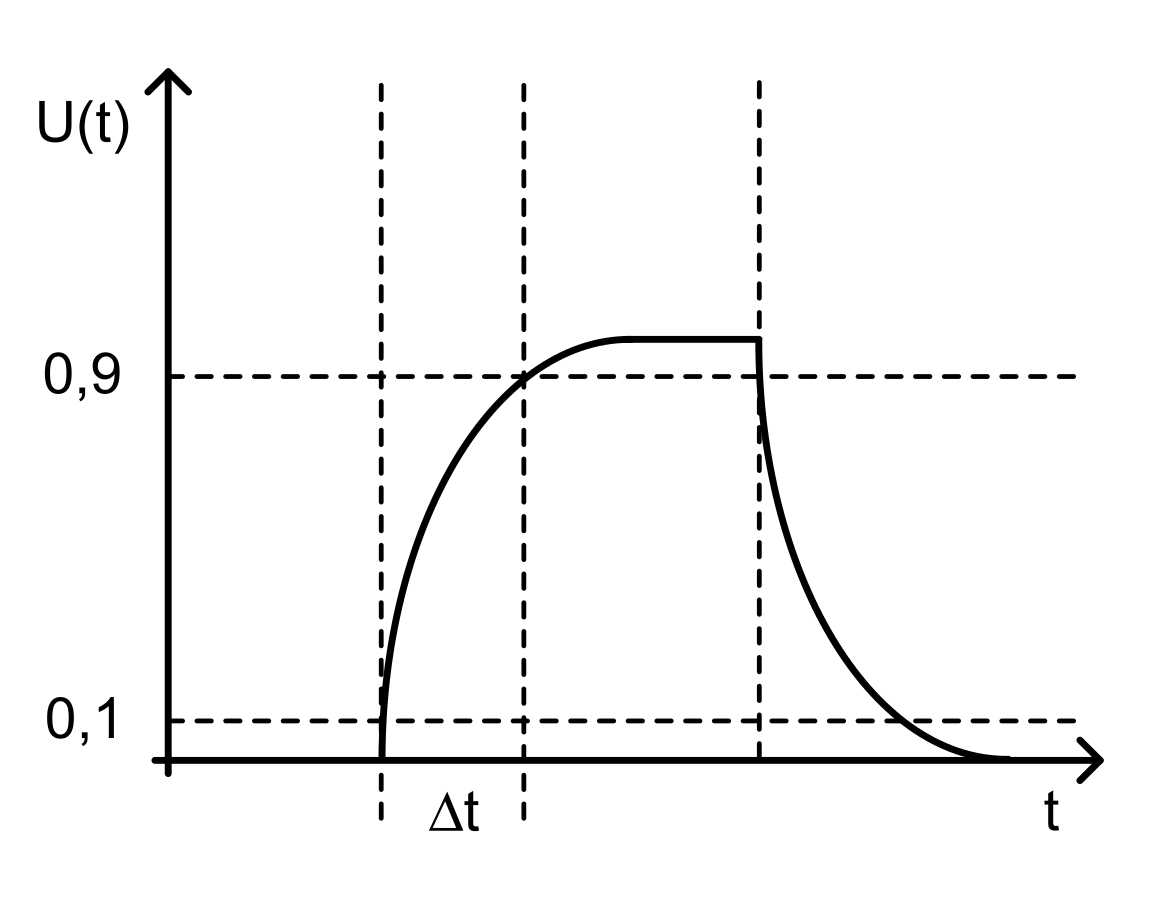
\includegraphics[width=0.5\textwidth]{rechteck_anstiegszeit.png}
        \caption{Rechteckimpuls mit endlicher Anstiegszeit; Abbildung 0.11 \cite{Praktikumsanleitung}}
\end{figure}\\
Statt der Bandbreite $B$ wird oft die Anstiegszeit $\Delta t$ angegeben, die ein Signal braucht, um von $10\%$ auf $90\%$ anzusteigen.
Näherungsweise gilt die Formel für exponentiell ansteigende Signale
\begin{align} 
        B\cdot \Delta t \approx 0.35
.\end{align} 
Da der Oszillograph auch eine Anstiegszeit besitzt, wird die echte Signalform verfälscht und es gilt
\begin{align} 
        \Delta t^2_\text{gemessen}=\Delta t^2_\text{Signal}+\Delta t^2_\text{Oszi}
.\end{align} 
%}}}

%{{{ Voraufgaben
\clearpage
\section{Voraufgaben}
\subsection{A}
Sie die Spannung $U\left(t\right)=U_0\sin \left(\omega t\right)$.
Dann ist
\begin{align} 
        U_{SS}&=2U_0&U_S&=U_0&U_{\text{eff}}&=\,\sqrt[]{\left\langle U_0^2\sin ^2\left(\omega t\right)\right\rangle }=\dfrac{U_0}{\,\sqrt[]{2}}
.\end{align} 

\subsection{B}
Mit $U_S=\SI{10}{V}$ folgt $U_{\text{eff}}=\,\sqrt[]{\left\langle \left(\SI{10}{V}\right)^2\right\rangle }=\SI{10}{V}$.

\subsection{C}
Es ist
\begin{align} 
        &&U_n&=U_0\dfrac{R_n}{R_n+R_i}&&\\
        \Leftrightarrow &&U_0&=\dfrac{U_n\left(R_n+R_i\right)}{R_n},&&
\end{align} 
Für $n  \in  \left[1,2\right]$ gilt dann
\begin{align} 
        \Rightarrow &&\dfrac{U_1\left(R_1+R_i\right)}{R_1}&=\dfrac{U_2\left(R_2+R_i\right)}{R_2}&&\\
        \Leftrightarrow &&I_1\left(R_1+R_i\right)&=I_2\left(R_2+R_i\right)&&\nonumber \\
        \Leftrightarrow &&I_1R_i-I_2R_i&=I_2R_2-I_1R_1&&\nonumber \\
        \Leftrightarrow &&R_i\left(I_1-I_2\right)&=U_2-U_1&&\nonumber \\
        \Leftrightarrow &&R_i&=\dfrac{U_2-U_1}{I_1-I_2}.&&
\end{align} 
Es ist $U_1=\SI{20}{V_{SS}}$ mit $I_1=0$ (unbelastet) und $U_2=\SI{10}{V_{SS}}$ mit $I_2=\tfrac{U_2}{R_2}=\SI{0.2}{A}$.
Damit ist 
\begin{align} 
        R_i&=\dfrac{\SI{10}{V_{SS}}-\SI{20}{V_{SS} }}{\SI{0}{A}-\SI{0.2}{A}}=\SI{50}{\ohm}.
\end{align} 

\subsection{E}
Für einen Tiefpass mit exponentiell ansteigender Flanke gilt
\begin{align} 
        U\left(t\right)&=U_0\left(1-\text{e}^{-t/\tau }\right)
.\end{align} 
Für die Zeit $\Delta $ die ein Rechtecksignal von $10\%$ auf $90\%$ aufsteigt gilt dann
\begin{align} 
        \Rightarrow &&U\left(t\right)&=0.1U_{\text{max}}=\left(1-\text{e}^{-t/\tau }\right)U_{\text{max}}&&\\
        \Rightarrow &&U\left(t+\Delta \right)&=0.9U_{\text{max}}=\left(1-\text{e}^{-\left(t+\Delta \right)/\tau }\right)U_{\text{max}}&&
\end{align} 
Daraus folgen
\begin{align} 
        &&0.1&=1-\text{e}^{-t/\tau }&&\\
        \Leftrightarrow &&\text{e}^{-t/\tau }&=0.9&&\nonumber \\
        \Leftrightarrow &&\tau &=-\dfrac{t}{\ln\left(0.9\right)}&&\nonumber \\
        \Leftrightarrow &&t&=-\ln(0.9)\tau. &&\label{eq:t}
\end{align} 
und 
\begin{align} 
        &&0.9&=1-\text{e}^{-\left(t+\Delta \right)/\tau }&&\\
        \Leftrightarrow &&\text{e}^{-\left(t+\Delta \right)/\tau }&=0.1&&\nonumber \\
        \Leftrightarrow &&\tau &=-\dfrac{t+\Delta }{\ln\left(0.1\right)}.&&\label{eq:delta}
\end{align} 
Die Zeitdifferenz ist dann $\Delta =\ln(0.9)\tau -\ln(0.1)\tau =\ln(9)\tau $.
Daraus folgt die Bandbreite
\begin{align} 
        B\cdot \Delta =\dfrac{1}{2\pi \tau }\ln(9)\tau \approx 0.35
.\end{align} 
%}}}

%{{{ Auswertung
\newpage
\section{Auswertung}
%}}}

\clearpage
\listoffigures
\listoftables

\bibliographystyle{plain}
\bibliography{refs}

%}}}

\end{document}
